% Chapter Template

\chapter{Software} % Main chapter title

\label{soft} % Change X to a consecutive number; for referencing this chapter elsewhere, use \ref{ChapterX}

\lhead{Chapter 4. \emph{Software}} % Change X to a consecutive number; this is for the header on each page - perhaps a shortened title



%----------------------------------------------------------------------------------------
%	SECTION 2
%----------------------------------------------------------------------------------------

\section{Introduction to Synrad3d}
\label{Synrad3d}
\srthree is a program built in Bmad. It was written by David Sagan using a photon scattering model developed by Gerry Dugan, both of them from Cornell University. 
 
\srthree  simulates the production and scattering of synchrotron radiation generated by an electron beam in a high energy machine. \citep{syn}. The \srthree program uses the Monte Carlo method for photon generation, scattering, and absorption calculations.
\subsection{Physics of Synrad3d}


This section is based on \cite{syn} 

To generate photons, a section of the machine is designated.  The user sets the total number of photons to be generated. \srthree calculates how many photons need to be generated within each machine element. The local bending field at the beam orbit is used to determine the photon spectrum.

Each photon is tracked from the point of origin to the point at which it hits the vacuum chamber wall. The angle of incidence relative to the local normal to the vacuum chamber is computed. The scattering probability is calculated, using this angle and the photon's energy. Using the value of this probability, the photon is either absorbed at this location, or scattered. If it is scattered, the scattering is taken to be elastic. That is, photon energy does not change. This ignores any florescence. Surface roughness, on the other hand is taken into account so there is a diffuse component to the scattering. Then the photon is tracked to the next hit on the vacuum chamber wall, and the probability of scattering is again computed. This process goes on until the photon is absorbed.
\subsubsection{Photon Generation}
Photon generation is based on the standard synchrotron radiation formulas, applicable for dipoles quadrupoles, and wigglers. The radiation is assumed to be incoherent.

\texttt{Synrad3D}\xspace  slices up each element longitudinally
and generates photons from each slice. The number of photons generated
in a slice weighted by the local probability of photon emission which
depends on the local orbit curvature.

Both circular and ``linear'' (that is, non-circular) machines can be
simulated.  In both cases, the orbit of the charged particle beam,
which may be non-zero, sets the centroid position and angular
orientation of the generated photons. Photon generation is based upon
the local field along the beam orbit. Thus, for example, off-axis
photons in a quadrupole will produce radiation. The beam orbit is
calculated from such things as the settings of steering elements,
element misalignments, etc. as given in the lattice file. For circular
machines, the beam orbit is the closed orbit. For linear machines, the
starting beam position as set in the lattice file is used in the orbit
calculation.

When a photon is generated at a given longitudinal position, the
beam's emittances and centroid are used so that the resulting photon
distribution mirrors the Gaussian positional distribution of the beam.
Horizontal/vertical coupling is taken into account in this
calculation. The photon energy distribution will be the standard
energy spectrum of photons generated in a bend.

A photon's initial angular orientation is generated by first using a
random number generator to generate an angular orientation using a
probability function that corresponds to the beam's angular
distribution. To this orientation, an angular offset out of the plane
of the bend is added where the offset is calculated using a random
number generator with a probability distribution based on the standard
angular spectrum of photons generated in a bend. There is no angular
offset added to the angle in the plane of the bend. The generated
photons will have the proper correlation between photon energy and
photon angle. Note that the plane of the bend may not be
horizontal. For example, the bend plane orientation for an offset beam
in a quadrupole will depend upon the offset.
\subsubsection{Photon Scattering} 

  \begin{figure}
  \centering
  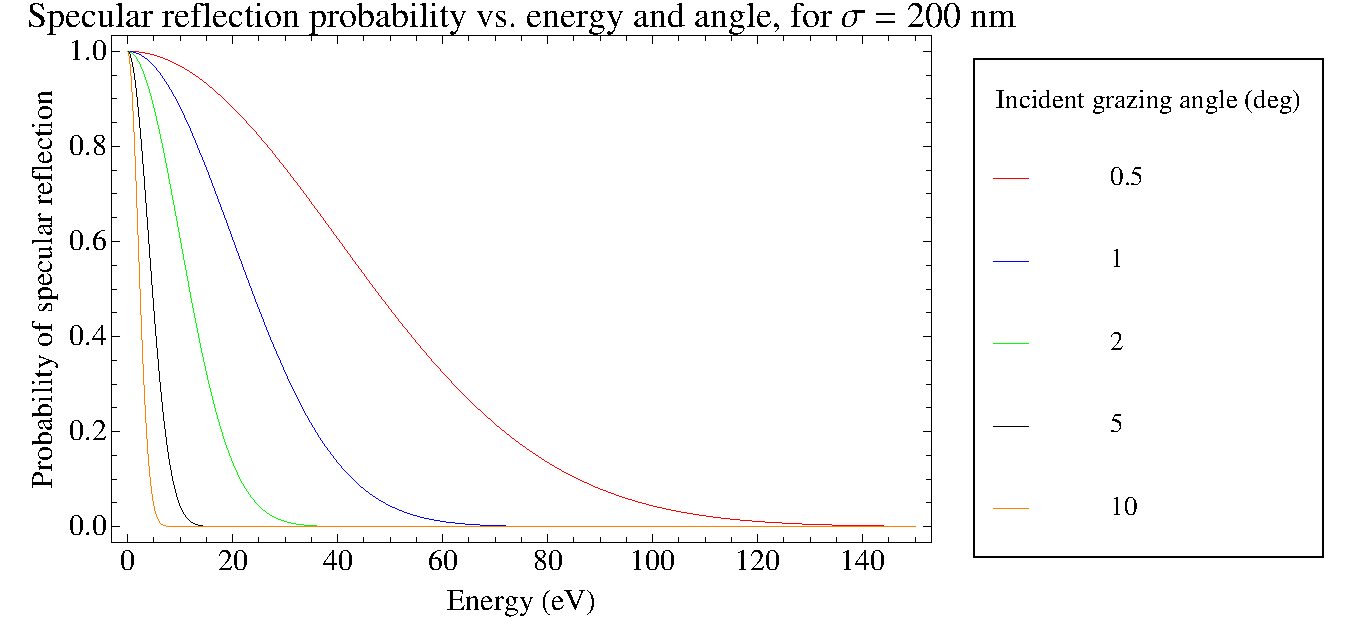
\includegraphics[width=6in]{Synrad3d/specular-probability.pdf}
  \caption[Specular reflection probability vs. photon energy and angle]
{\label{f:spec.prob}
Specular reflection probability~\cite{b:beckmann}, vs. photon energy
and angle, for an rms surface roughness of 200 nm.}
  \end{figure}
   
Simulated photons are tracked until they hit the wall, where the
probability of being scattered, and the scattering angle, are
determined by their energy and angle of incidence.  This section
describes the scattering model.

Generally, the probability of specular reflection of a photon from a
rough surface depends on the the rms surface roughness $\sigma$, the
photon wavelength $\lambda$, and the grazing angle. An explicit
formula for this probability is~\cite{b:beckmann}
   \begin{equation}
P_{\textrm{spec}}=\textrm{e}^{-g(x,x)},
\end{equation}
in which
   \begin{equation}
g(x,y)=\frac{4\pi^{2}\sigma^{2}(x+y)^{2}}{\lambda^{2}}
  \end{equation}
where $x$ is the cosine of the incident polar angle, and $y$ is the
cosine of the scattered polar angle. For a typical technical vacuum
chamber surface, the rms surface roughness $\sigma \gtrsim 200$ nm is
greater than most of the X-ray wavelengths of interest, for all except
the lowest energy photons. In this regime, except at very small
grazing angles, diffuse scattering from the surface dominates over
specular reflection. This is illustrated in Fig.~\ref{f:spec.prob}.
The theory of diffuse scattering of electromagnetic waves from random
rough surfaces is a well-developed subject, and is covered in detail
in references \cite{b:beckmann} and \cite{b:ogilvy}. The model we use
assumes a Gaussian distribution for both the surface height variations
(rms $\sigma$) and for the transverse distribution (equal in both
transverse directions, with autocorrelation coefficient $T$).
  \begin{figure}
  \centering
  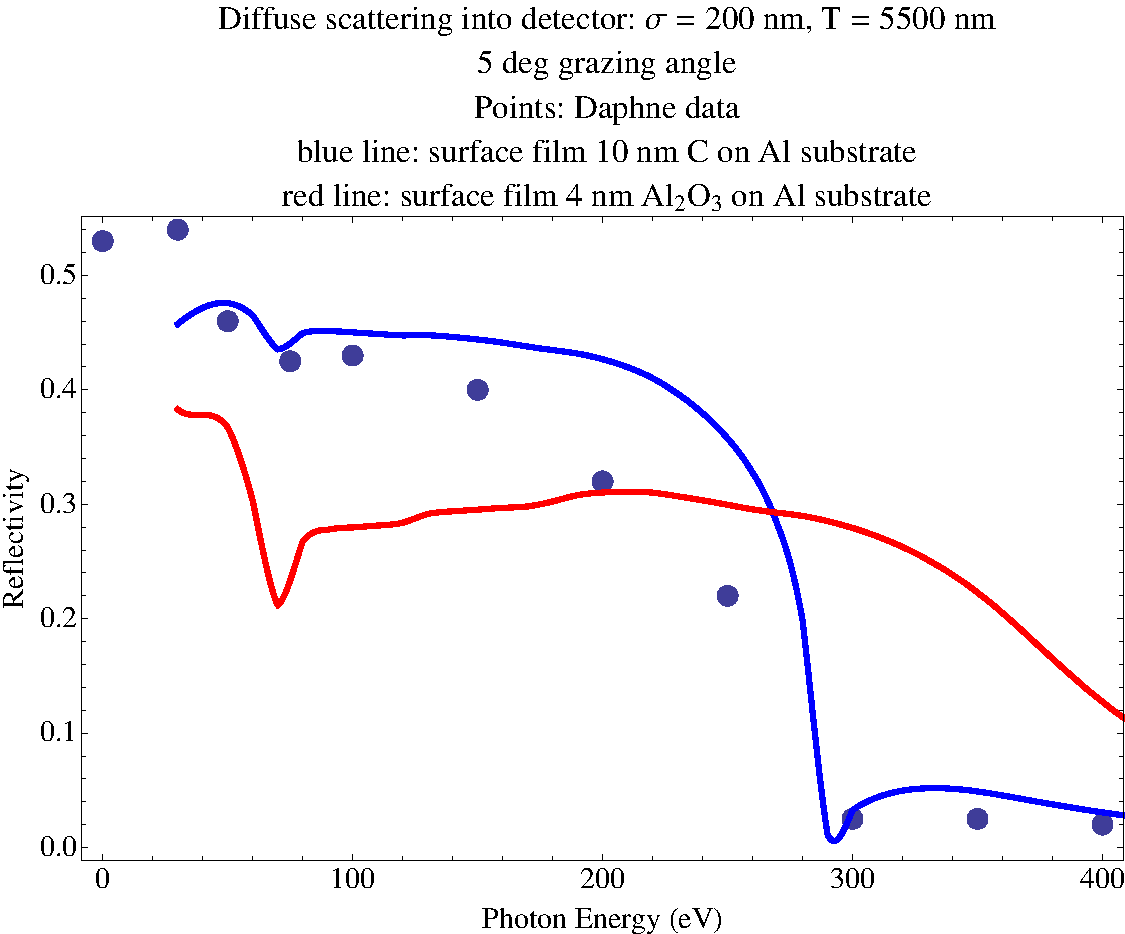
\includegraphics[width=4.5in]{Synrad3d/Daphne-fit-5-deg}
  \caption{\label{f:Daphne.fit.5.deg}
   Diffuse scattering at 5 deg from a surface layer on an aluminum substrate: comparison of data and model}
   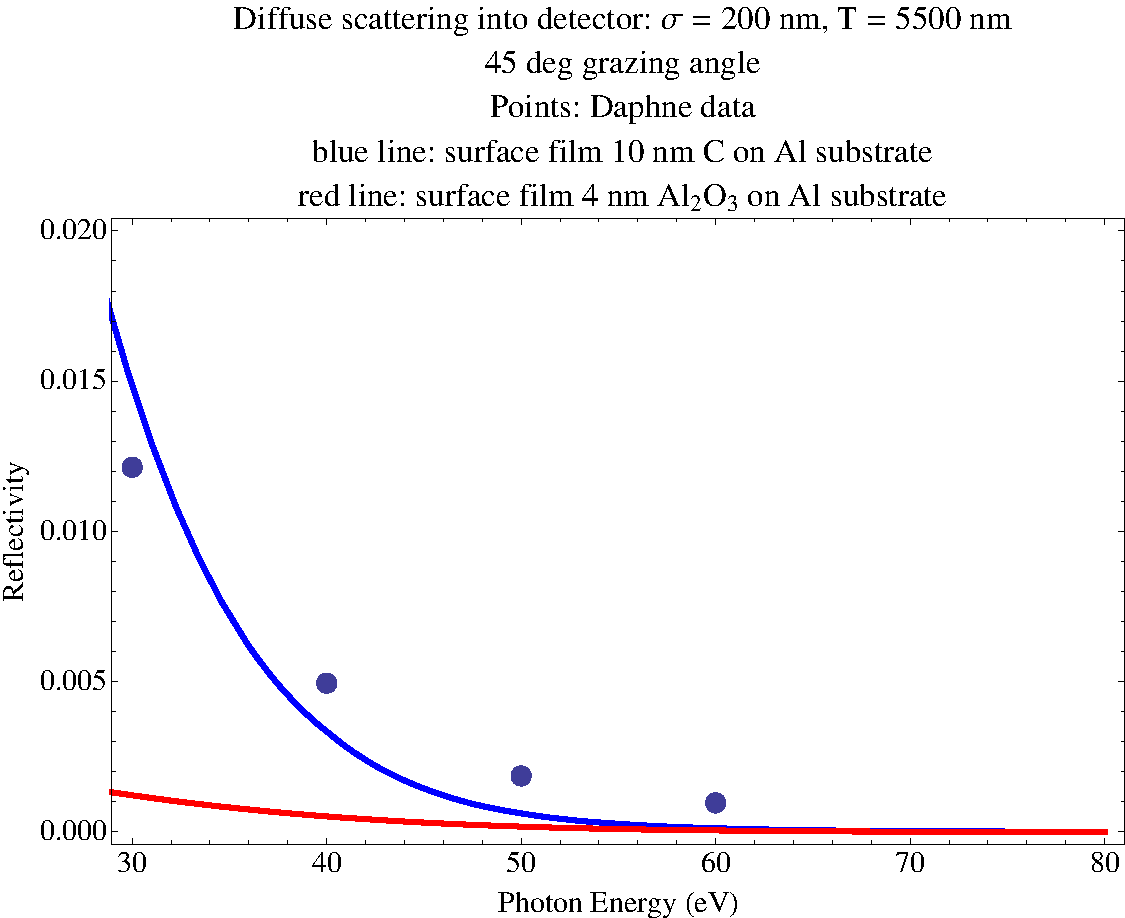
\includegraphics[width=4.5in]{Synrad3d/Daphne-fit-45-deg}
   \caption{\label{f:Daphne.fit.45.deg}
   Diffuse scattering at 45 deg from a surface layer on an aluminum substrate: comparison of data and model}
   \end{figure}

  \begin{figure}
  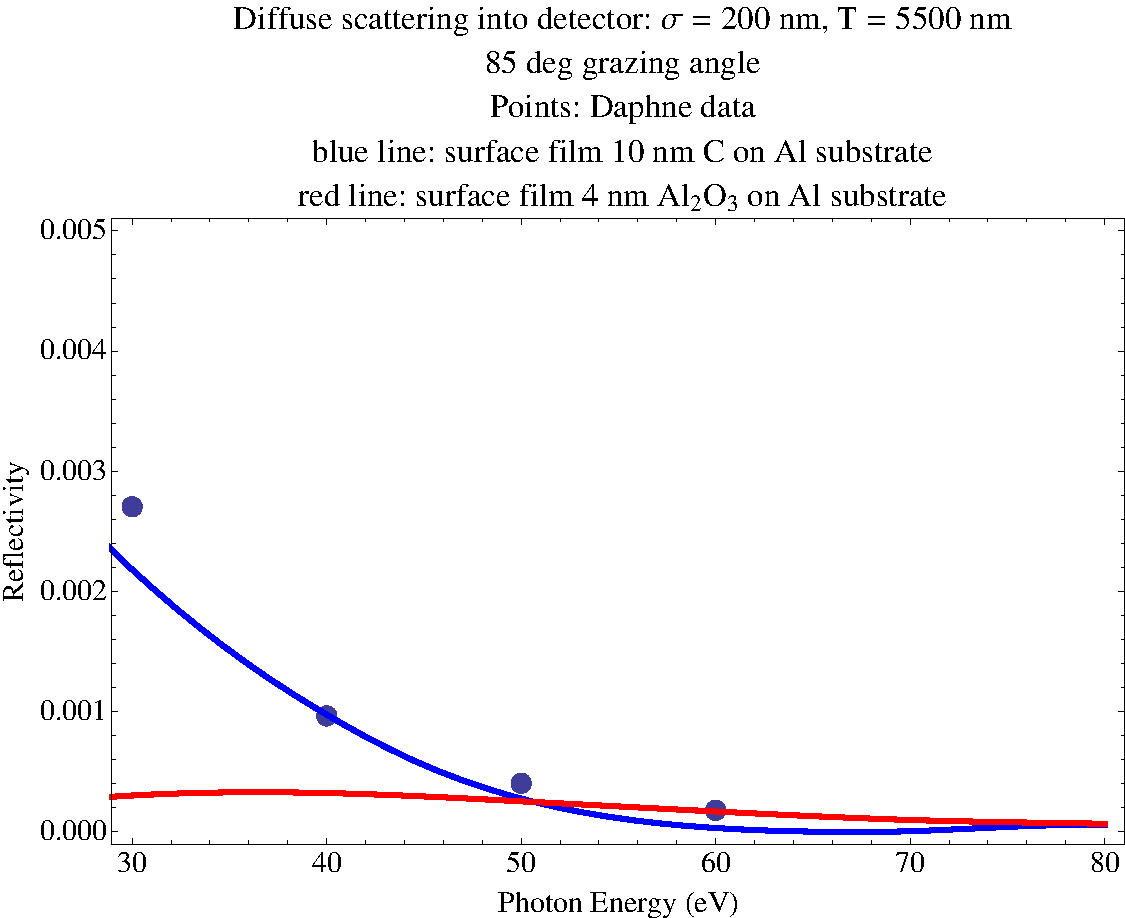
\includegraphics[width=4.5in]{Synrad3d/Daphne-fit-85-deg}
   \caption{\label{f:Daphne.fit.85.deg}
   Diffuse scattering at 85 deg from a surface layer on an aluminum substrate: comparison of data and model}
  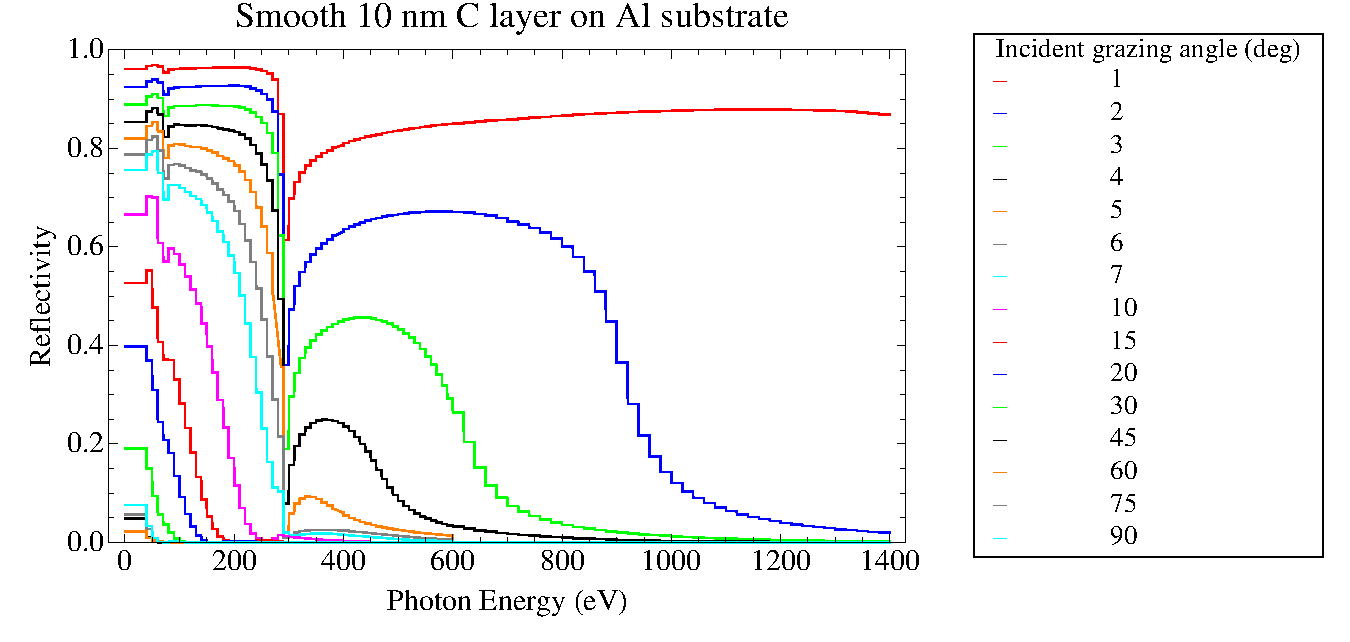
\includegraphics[width=6in]{Synrad3d/Smooth-surface-reflectivity}
   \caption[Smooth surface reflectivity for a 10 nm C film on Al substrate]
   {\label{f:Smooth.surface.reflectivity}
   Smooth surface reflectivity for a 10 nm C film on Al substrate: from \cite{b:henke}}
  \centering
   \end{figure}

      \begin{figure}
  \centering
  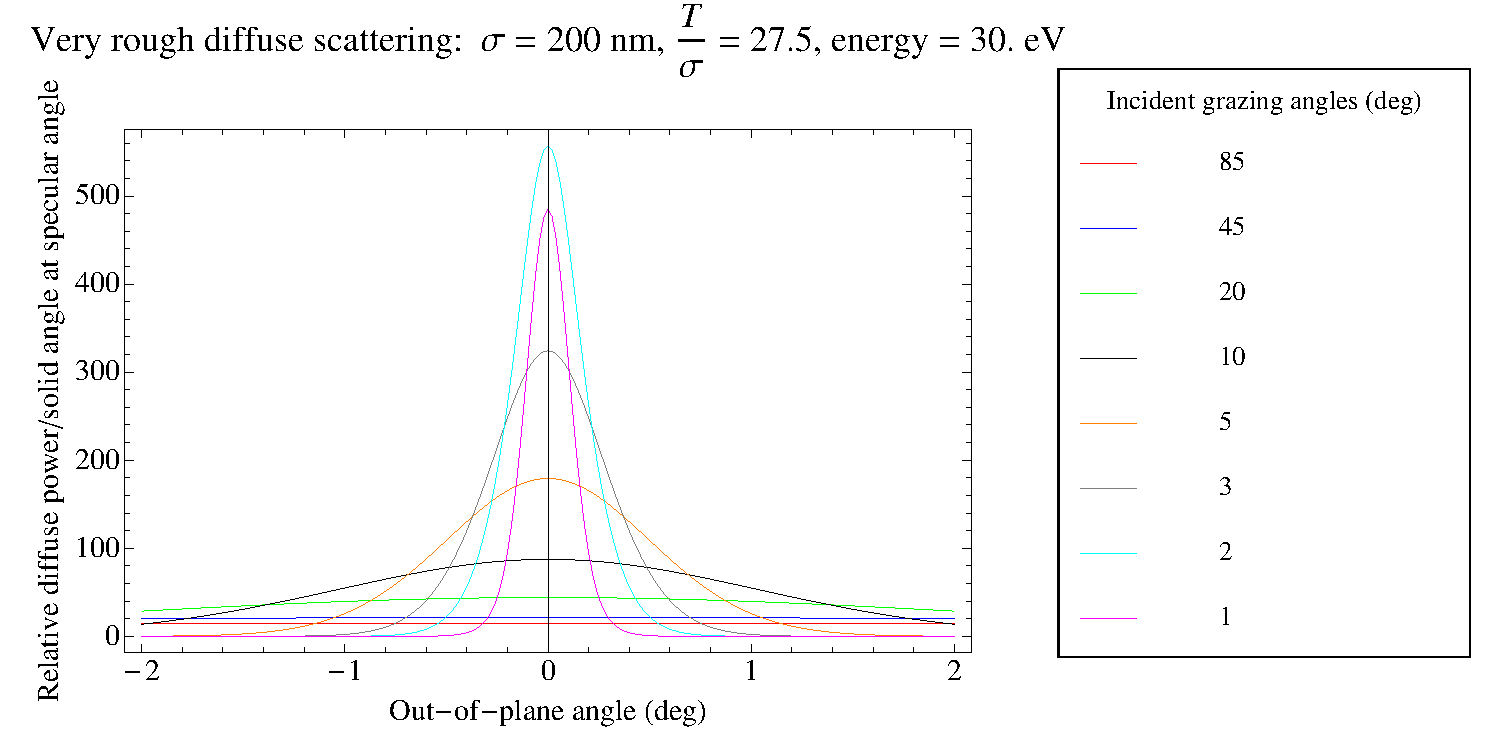
\includegraphics[width=6in]{Synrad3d/Diffuse-out-of-plane-30ev}
   \caption{   \label{f:Diffuse.out.of.plane.30ev}
   Diffuse scattering out-of-plane angular distributions for 30 eV photons}
 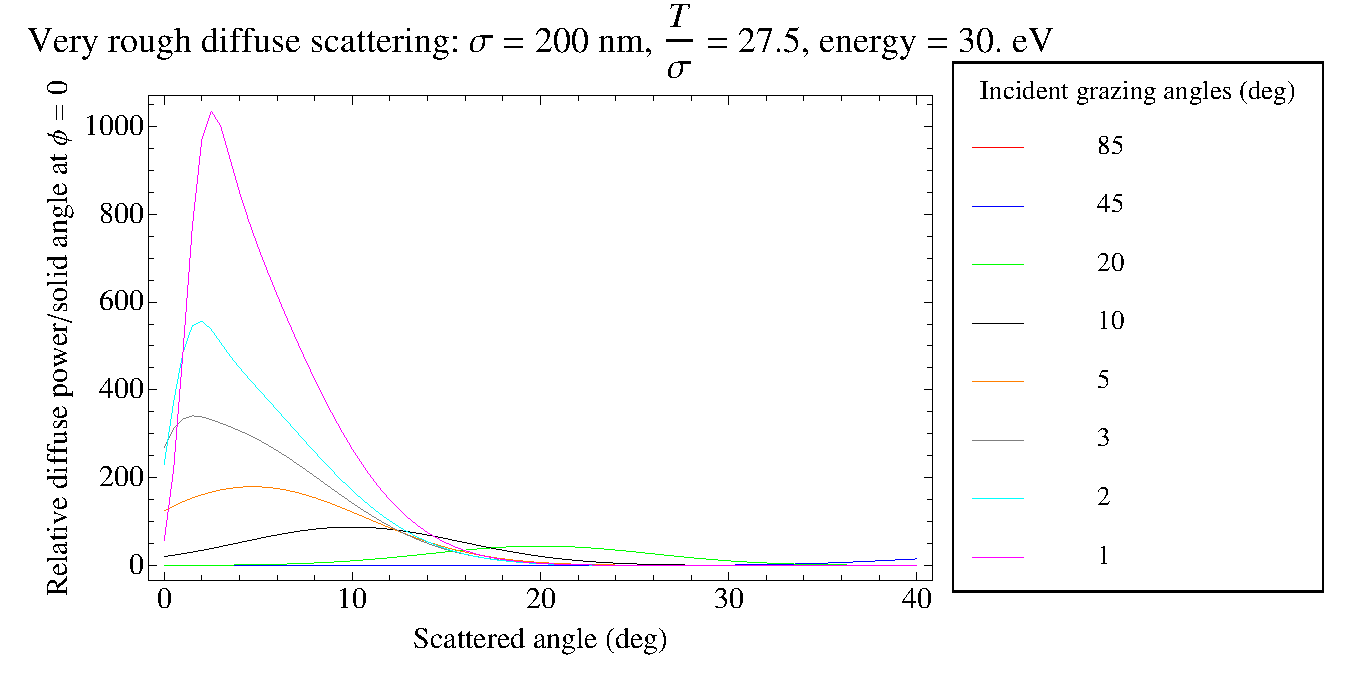
\includegraphics[width=6in]{Synrad3d/Diffuse-polar-30ev}
   \caption{   \label{f:Diffuse.polar.30ev}
   Diffuse scattering polar angular distributions for 30 eV photons}
   \end{figure}

  \begin{figure}
  \centering
  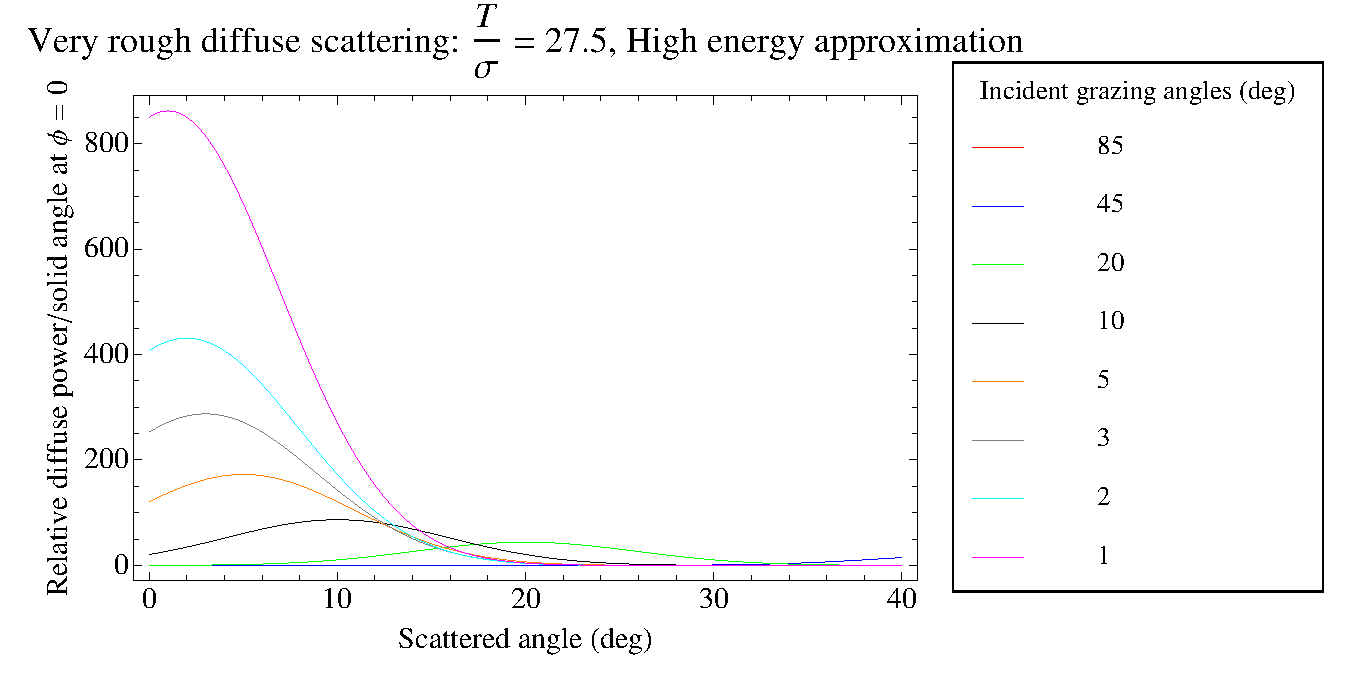
\includegraphics[width=6in]{Synrad3d/Diffuse-polar-HE}
   \caption{   \label{f:Diffuse.polar.HE}
    Diffuse scattering polar angular distributions for high energy photons}
  \centering
  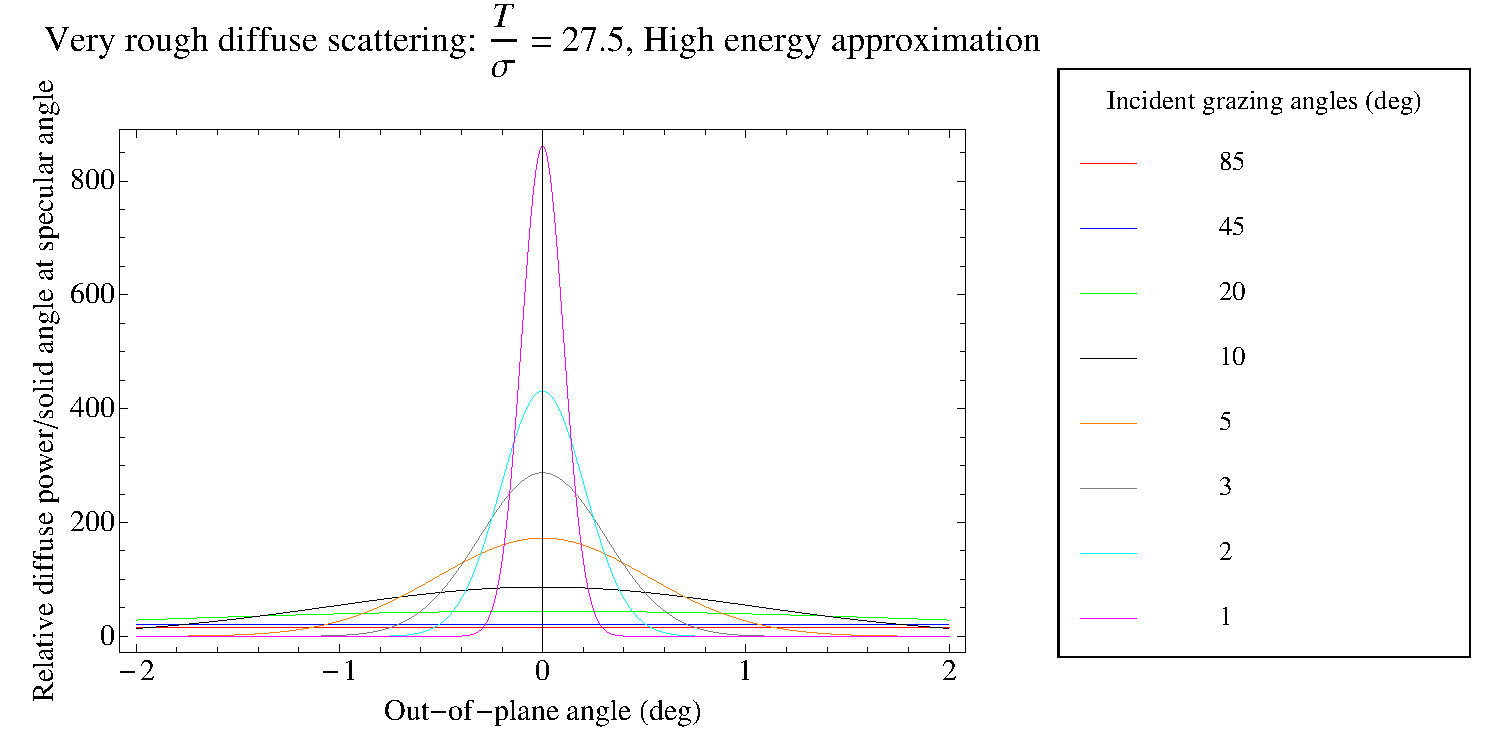
\includegraphics[width=6in]{Synrad3d/Diffuse-out-of-plane-HE}
   \caption{   \label{f:Diffuse.out.of.plane.HE}
   Diffuse scattering out-of-plane angular distributions for high energy photons}
   \end{figure}
   
The most general expression for the diffusely scattered power is
complex, and involves an infinite sum.  However, the expression
simplifies substantially in the limit $g(x,y)\gg 1.$ For very rough
surfaces corresponding to technical vacuum chambers, for which
typically $\sigma \gg \lambda$, this condition is satisfied over much
of the region of interest. In this limit, the diffusely scattered
power per unit solid angle is given by
  \begin{equation}
  \frac{d P_{\textrm{diff}}}{d \Omega} = P_{0}\frac{\left<R\right>}{4\pi y}
  \frac{(1+xy)^{2}}{(x+y)^{4}}\tau^{2}\textrm{e}^{-\frac{(2-x^{2}-y^{2})
  \tau^{2}}{4(x+y)^{2}}}(1-a\cos\phi)^{2}\textrm{e}^{b\cos\phi},
  \label{Eq.diffuse.power}
  \end{equation}
with
   \begin{align}
   a&=\frac{h(x,y)}{1+xy}, \\
   b&=\frac{2h(x,y)\tau^{2}}{4(x+y)^{2}}, \\
   h(x,y)&=\sqrt{1-(x^{2}+y^{2})+x^{2}y^{2}}.
   \end{align}
In this expression, $P_{0}$ is the incident power, and $\left<R\right>$ is the smooth-surface reflectivity, which is determined by the atomic structure of the surface material. $\phi$ is the scattering angle out of the plane of incidence. Note that the relative power depends on the ratio $\tau=T/\sigma$, and not on the $T$ or $\sigma$ separately.

The smooth-surface reflectivity $\left<R\right>$ depends on the atomic structure of the surface materials (including any thin layers which may be deposited on the surface). The surface roughness parameters $\sigma$ and $T$ depend on the geometry of the surface deviations from a perfect plane. These parameters may be determined from inspection of the vacuum chamber surface, for example, using an atomic force microscope.

To derive a working model for the smooth surface reflectivity and the surface parameters for a typical vacuum chamber surface, we have relied on measurements~\cite{b:mehne} of X-ray scattering from an aluminum vacuum chamber surface made at DAPHNE. For these measurements, the rms surface roughness of the sample was reported to be 200 nm.

The theory of diffuse scattering discussed above has been used, together with smooth surface reflectivity results taken from an X-ray database~\cite{b:henke}, to predict the scattering and compare with the measurements. From these comparisons, the best-fit value for the transverse autocorrelation parameter, $T$, was found to be 5500 nm. In addition, it was found that the smooth-surface reflectivity corresponding to a 10 nm carbon film on an aluminum substrate was needed to fit the data. The assumption of an aluminum oxide surface film was not consistent with the data. The data and the corresponding fits are shown in Fig.~\ref{f:Daphne.fit.5.deg},
\ref{f:Daphne.fit.45.deg}, and \ref{f:Daphne.fit.85.deg}.

With the smooth-surface reflectivity determined, and the surface
parameters established, the scattering model in \srthree is
completely determined. The model currently in use has a smooth-surface
reflectivity illustrated in
Fig.~\ref{f:Smooth.surface.reflectivity}. Diffuse
scattering distributions for 30 eV photons are shown in
Fig.~\ref{f:Diffuse.polar.30ev} and
Fig.~\ref{f:Diffuse.out.of.plane.30ev}. At this low photon
energy, the approximation $g(x,y)\gg 1$ does not hold in general, and
the full diffuse scattering formalism is used to compute these
distributions. Diffuse scattering distributions for high energy
photons, for which $g(x,y)\gg 1$ are shown in
Fig.~\ref{f:Diffuse.polar.HE} and
Fig.~\ref{f:Diffuse.out.of.plane.HE}. These distributions
have been computed from Eq.~\ref{Eq.diffuse.power}.

\subsection{Input Files}
The input files used by \srthree are the following:
\subsubsection*{Synrad3d Main Input File}
This file should be specified on the command line that invokes synrad3d, if it is not specified, it will select the default name "synrad3d.init". This file contains the parameters of the simulation
\begin{itemize}
\item The region where radiation is produced specified by the index numbers of elements in the lattice.
\item The direction in which the photons are travelling when initially created.
\item The minimun number of photons that need to be generated before \srthree will stop the simulation
\item the number of photons generated throughout the radiation production region.
\item The minimun distance to track the particle beam between emission points.
\item The particle beam size.
\item The lattice file defining the optics of the accelerator.
\item The wall file defining the vacuum chamber's details.
\item The name of the output file.
\item The surface roughness for the default surface.
\item The surface roughness correlation for the default surface.
\item The surface reflection file for non-default surface.
\item The minimun and maximun initial energy values to be filtered by \srthree .
\end{itemize}
There are other parameters that can be specified in the SMIF, but are not mentioned here, because they are not relevant to my work.

\subsubsection*{Lattice File}
This file cointains the complete description of the elements of the lattice, defining the optics of the machine. This file must be specified in the SMIF.
\subsubsection*{Vacuum Chamber Wall Definition}
The file specified in the SMIF defines the cross section of the vacuum chamber's wall at a number of longitudinal positions.
\subsubsection*{Chamber Surface Reflectivity}
The reflectivity of the vacuum chamber wall can be described on the surface reflection file specified in the SMIF. If no file is specified \srthree will use the default reflectivity, which  is based on the refletivity of a Carbon film on Aluminum substrate. 

\subsection{Output Files}

\subsubsection*{Synrad3d Main Input File}
The name of this file must be specified in the SMIF. This file contains the information in the SMIF and the data generated for ech photon. The information of the photon consists in:
\begin{itemize}
\item The number of the photon.
\item The number of times the photon hit the wall.
\item The photon's energy.
\item The position where the photon was generated.
\item The position where the photon was absorbed.
\item The distance traveled by the photon.
\item The type of elemet of the lattice that absorbed the photon.
\end{itemize}

Once again there a couple of elements left out because they are irrelevant to this work.

\subsubsection*{Output Table}

In order to make easier to read and manipulate the data, the photons information is also written in a table format which keeps the same name as the SMOF with the extension .dat$\_$table.
 

%----------------------------------------------------------------------------------------
%	SECTION 1
%----------------------------------------------------------------------------------------

\section{Bmad}

Bmad, which was build in 1996 at Cornell University's Laboratory for Elementary Particles Physics, is  a sub routine library for relativistic charged particles and X-Ray simulations in high energy accelerators and storage rings. Bmad subroutine has an object oriented aproach and is written in Fortran90. The main objectives of this project are:
	
\begin{itemize}
\item Cut down on the time needed to develop programs.
\item Minimize computation times.
\item Cut down on programming errors,
\item Provide a simple mechanism for lattice function calculations from within control system programs.
\item Provide a flexible and powerful lattice input format.
\item Standardize sharing of lattice information between programs.
\end{itemize}

Bmad diverse routines are capable of doing many things, such as simulating Wake fields and radiation stimulation, calculating transfer matrices, emittances, Twiss parameters,
dispersion, coupling, etc., and include various tracking algorithms including Runge-Kutta and symplectic integration. 


We are particularly interested in a set of routines used to build a program called \texttt{Synrad3D}\xspace , which is used to track both produced and scattered photons from SR in a high energy machine. This particular program is described in \ref{Synrad3d}


%--------------------------------------------------------------------------------------------
\section{Tools}
Given the nature of routines described in \ref{Synrad3d}, using enough photons to obtain statistically valid results, running this program would take months in a regular commercial computer. To surpass this limitation we were grated access to the {\it Lxplus} computing cluster at CERN.
\subsection{Lxplus}
The Lx Public Login Service or Lxplus is a login service offered to all CERN users. This cluster consists in several public machines running SLC5 in 64 bit mode, where all interactive and batch systems are built on top of the CERN standart Unix Enviroment. There is a wide range of shells available, that can be sorted in two groups: the C-shell like and the Bourne-shell like. We used Bash because of the full Linux based facilities. Since this machines are not to be used to store data a Workspace was made in the AFS file system that is accesible through normal system commands. Running CPU intense jobs in those machines is prohibited. 
\subsection{Lxbatch}
To run CPU intense jobs we used Lxbatch that currently consists of around 30,000 CPU cores running platform LSF\textregistered. This service is open to all CERN users and its aim is to share teh resources fairly between all CERN experiments. So the amount of resources we can use depends on how much other experiments are using. 
There ar different queues to which jobs can be send, one should select the queue considering the processing time the job will requiere, there are queues in the range 8 minutes to 2 weeks. we ran our jobs in the 1 week queue. 



